% Fig: modules of the implementation and their main functions
\documentclass[border=2pt]{standalone}
\usepackage{mathptmx}
\usepackage{tikz}
\usetikzlibrary{arrows.meta,positioning,fit,backgrounds}
\begin{document}
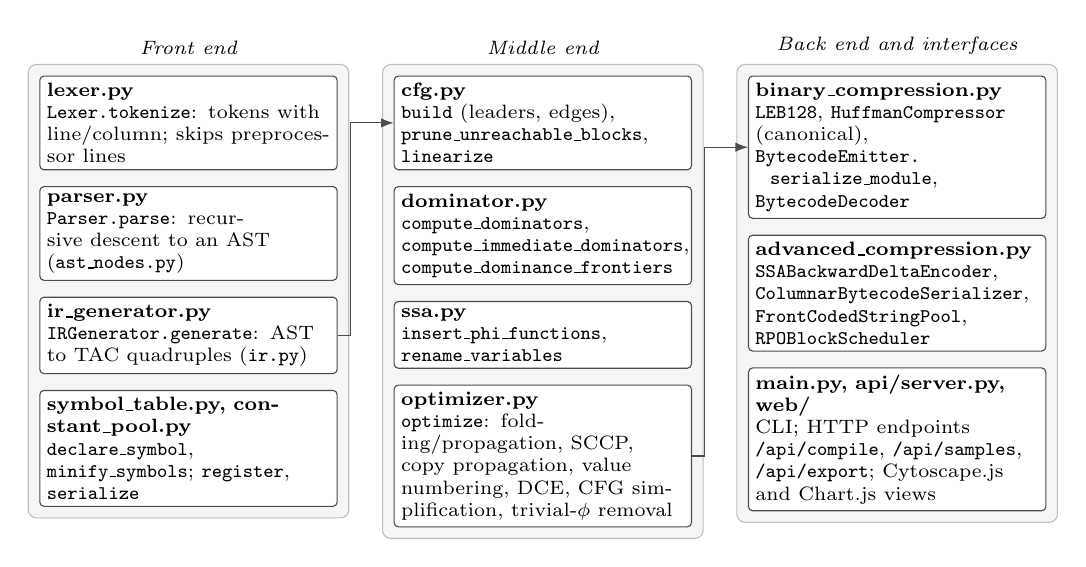
\begin{tikzpicture}[
  font=\scriptsize,
  mod/.style={draw=black!70, rounded corners=1.5pt, fill=white, align=left, text width=36mm, inner sep=2.5pt, anchor=north},
  lane/.style={draw=black!25, rounded corners=3pt, fill=black!4, inner sep=4pt},
  arr/.style={-{Latex[length=1.6mm]}, black!70}]
  % column 1: front end
  \node[mod] (lex) at (0,0) {\textbf{lexer.py}\\ \texttt{Lexer.tokenize}: tokens with line/column; skips preprocessor lines};
  \node[mod, below=2mm of lex.south, anchor=north] (par) {\textbf{parser.py}\\ \texttt{Parser.parse}: recursive descent to an AST (\texttt{ast\_nodes.py})};
  \node[mod, below=2mm of par.south, anchor=north] (gen) {\textbf{ir\_generator.py}\\ \texttt{IRGenerator.generate}: AST to TAC quadruples (\texttt{ir.py})};
  \node[mod, below=2mm of gen.south, anchor=north] (sym) {\textbf{symbol\_table.py, constant\_pool.py}\\ \texttt{declare\_symbol}, \texttt{minify\_symbols}; \texttt{register}, \texttt{serialize}};
  % column 2: middle end
  \node[mod] (cfg) at (45mm,0) {\textbf{cfg.py}\\ \texttt{build} (leaders, edges), \texttt{prune\_unreachable\_blocks}, \texttt{linearize}};
  \node[mod, below=2mm of cfg.south, anchor=north] (dom) {\textbf{dominator.py}\\ \texttt{compute\_dominators}, \texttt{compute\_immediate\_dominators}, \texttt{compute\_dominance\_frontiers}};
  \node[mod, below=2mm of dom.south, anchor=north] (ssa) {\textbf{ssa.py}\\ \texttt{insert\_phi\_functions}, \texttt{rename\_variables}};
  \node[mod, below=2mm of ssa.south, anchor=north] (opt) {\textbf{optimizer.py}\\ \texttt{optimize}: folding/propagation, SCCP, copy propagation, value numbering, DCE, CFG simplification, trivial-$\phi$ removal};
  % column 3: back end and interfaces
  \node[mod] (bin) at (90mm,0) {\textbf{binary\_compression.py}\\ \texttt{LEB128}, \texttt{HuffmanCompressor}\\ (canonical), \texttt{BytecodeEmitter.}\\ \texttt{\ \ serialize\_module}, \texttt{BytecodeDecoder}};
  \node[mod, below=2mm of bin.south, anchor=north] (adv) {\textbf{advanced\_compression.py}\\ \texttt{SSABackwardDeltaEncoder},\\ \texttt{ColumnarBytecodeSerializer},\\ \texttt{FrontCodedStringPool},\\ \texttt{RPOBlockScheduler}};
  \node[mod, below=2mm of adv.south, anchor=north] (ui) {\textbf{main.py, api/server.py, web/}\\ CLI; HTTP endpoints \texttt{/api/compile}, \texttt{/api/samples}, \texttt{/api/export}; Cytoscape.js and Chart.js views};
  % lanes
  \begin{scope}[on background layer]
    \node[lane, fit=(lex)(sym), label={[font=\scriptsize\itshape]above:Front end}] {};
    \node[lane, fit=(cfg)(opt), label={[font=\scriptsize\itshape]above:Middle end}] {};
    \node[lane, fit=(bin)(ui), label={[font=\scriptsize\itshape]above:Back end and interfaces}] {};
  \end{scope}
  \draw[arr] (gen.east) -- ++(1.6mm,0) |- (cfg.west);
  \draw[arr] (opt.east) -- ++(1.6mm,0) |- (bin.west);
\end{tikzpicture}
\end{document}
